\section{Demo}

\begin{frame}{Demo}
    \begin{columns}[T]
        \begin{column}{0.5\textwidth}
            This demo aims to showcase the feasibility of self-debugging by large language models (LLMs).\\
            The current implementation utilizes zero-shot prompting and ChatGPT Turbo 3.5, with code available on GitHub at this \href{https://github.com/tqtensor/wolverine}{link}.\\
            \vspace{0.5cm}
            In this example there are two bugs:
            \begin{enumerate}
                \item `subtract\_number' function is not defined.

                \item The return must be `result'.
            \end{enumerate}
        \end{column}
        \begin{column}{0.5\textwidth}
            \begin{figure}[!htb]
                \centering
                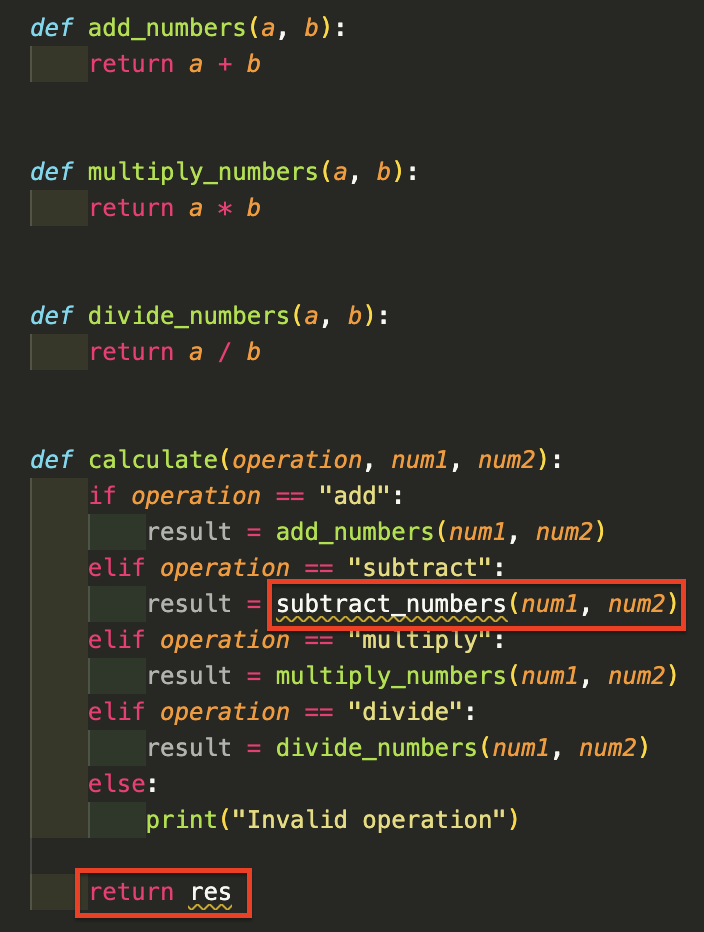
\includegraphics[width=0.7\textwidth]{img/demo}
                \captionsetup{font=small,labelformat=empty}
                \caption{Example of Python bug.}
            \end{figure}
        \end{column}
    \end{columns}
\end{frame}
